% !TEX root = ../PolycopiePremiere2627.tex
%%%%%%%%%%%%%%%%%%%%%%%%%%%%%%%%%%%%%%%%%%%%%%%%%%%%%%%%%%%%%%%%%%%%%%%%%%%%%%%%
% Contenu initial repris de Louis Paternault --- http://ababsurdo.fr
%
% Publié sous licence Creative Commons Attribution-ShareAlike 4.0 International (CC BY-SA 4.0)
% http://creativecommons.org/licenses/by-sa/4.0/deed.fr
%%%%%%%%%%%%%%%%%%%%%%%%%%%%%%%%%%%%%%%%%%%%%%%%%%%%%%%%%%%%%%%%%%%%%%%%%%%%%%%%

\chapter{Suites géométriques}

\noindent\textbf{Activité}

On définit la suite $v$ par le schéma suivant.

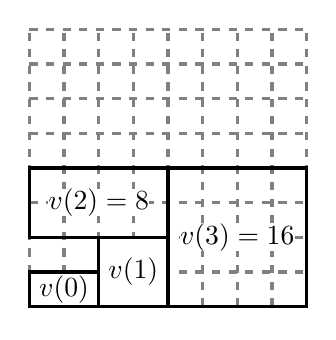
\begin{tikzpicture}[scale=.44,very thick]
    \draw[dashed, gray] (0, 0) grid (8, 8);
    \draw (0, 2) rectangle (4, 4) node[midway, fill=white, inner sep=0pt]{$v(2)=8$};
    \draw (4, 0) rectangle (8, 4) node[midway, fill=white, inner sep=0pt]{$v(3)=16$};
    \draw[fill=white](2, 0) rectangle ++(2, 2) node[midway]{$v(1)$};
    \draw[fill=white](0, 0) rectangle ++(2, 1) node[midway]{$v(0)$};
\end{tikzpicture}%
\begin{minipage}[b]{.7\textwidth}
    \begin{enumerate}
        \item Donner $v(0)$ et $v(1)$.
        \item Quel calcul doit être fait à chaque étape pour calculer le terme suivant ?\\
        \item Calculer :

        \begin{tabularx}{\linewidth}{XXX}
            $v(4)=\ldots$ ;&
            $v(5)=\ldots$ ;&
            $v(7)=\ldots$ ;\\
            $v(25)=\ldots$ ;&
            $v(100)=\ldots$ ;&
            $v(-1)=\ldots$.\\
        \end{tabularx}
        \item Exprimer $v(n+1)$ en fonction de $v(n)$.
    \end{enumerate}
\end{minipage}

\bigskip

Une suite est géométrique si on passe au terme suivant en multipliant (ou divisant) toujours le même nombre.

\Dfn{Une suite $u$ est dite \textcolor{J1}{géométrique} s'il existe un réel $q$, appelé \textcolor{J1}{raison}, tel que pour tout $n\in\mathbb{N}$, on ait : \textcolor{J1}{$u_{n+1}=q\times u_n$}.

Habituellement, une suite géométrique est définie par la donnée de \textcolor{J1}{son premier terme et sa raison}.}

\Exemple[avec calculatrice]{\label{ex:calculGeo}
\begin{enumerate}
    \item Donner les cinq premiers termes (arrondis au centième) de la suite géométrique $u$ de premier terme $u_0=2$ et de raison \numprint{2,5}.
    \item La suite $v$ est géométrique, et on sait que $v_3=2$ et $v_5=18$. Déterminer la raison positive, puis calculer $v_4$, $v_6$, et $v_2$.
\end{enumerate}}

\Exemple{\label{ex:graphGeo}
Représenter graphiquement (de couleur différente) les deux suites de l'exemple \ref{ex:calculGeo}. Les suites sont-elles arithmétiques ?
\begin{center}
    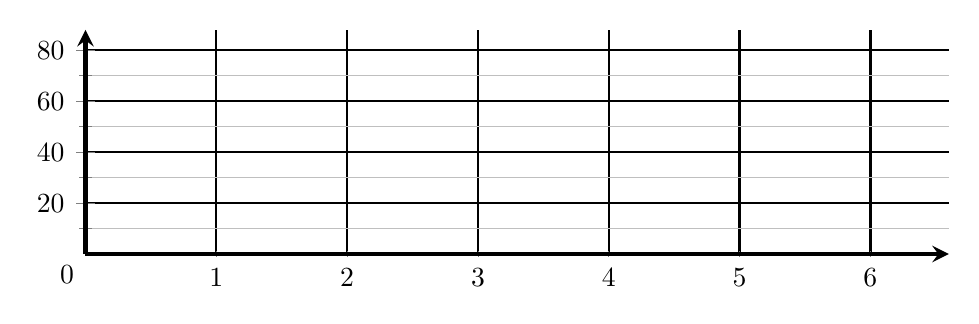
\begin{tikzpicture}[scale=1,very thick]
        \begin{axis}[
                yscale=.5,
                xscale=1.6,
                xmin=0,
                xmax=6,
                ymin=0,
                ymax=80,
                ultra thick,
                axis lines=middle,
                enlargelimits=upper,
                minor y tick num=1,
                major grid style={black, thick},
                grid=both,
                clip=false,
            ]
            \draw (axis cs:0, 0) node[below left]{$0$};
        \end{axis}
    \end{tikzpicture}%
\end{center}}

\Prp{On dit que les termes d'une suite géométrique suivent un modèle de \textcolor{J1}{croissance exponentielle}.}

\pagebreak

\Prp{Une suite géométrique $u$ de premier terme strictement positif est :
\begin{itemize}
    \item \emph{croissante} si et seulement si sa raison est \textcolor{J1}{$q>1$} ;
    \item \emph{décroissante} si et seulement si sa raison est \textcolor{J1}{$0<q<1$} ;
    \item \emph{constante} si sa raison est \textcolor{J1}{$q=1$}.
\end{itemize}}

\Exemple{Déterminer les variations des deux suites $u$ et $v$ de l'exemple \ref{ex:calculGeo}.}

\Prp{
\begin{itemize}
    \item Pour tout $n$ et $p$ de son domaine de définition, on a : \[\textcolor{J1}{u_n=u_p\times q^{n-p}}\]
    \item En particulier, si $u$ est définie sur $\mathbb{N}$, pour tout $n\in\mathbb{N}$, on a : \[\textcolor{J1}{u_n=u_0\times q^n}\]
\end{itemize}}

\Exemple{On reprend les suites $u$ et $v$ de l'exemple \ref{ex:calculGeo}. Sans utiliser le module suite de la calculatrice, déterminer $u_{100}$ et $v_{100}$.}

\Exemple[D'après le sujet zéro de l'épreuve anticipée de mathématiques aux baccalauréats général et technologique 2026]{
Victor sort un plat du four. La température du plat est alors égale à 180\,\textdegree C. Il place ce plat dans une pièce dont la température est égale à 25\,\textdegree C. Le plat refroidit.

Le plat ne pourra être servi que lorsque sa température sera devenue inférieure ou égale à 40\,\textdegree C.

Trois minutes après la sortie du four, on mesure que la température du plat est égale à 105\,\textdegree C.

Pour tout entier naturel $n$ on note $U_n$, la différence entre la température du plat et la température de la pièce, $n$ minutes après la sortie du four.

Exemple : 3 minutes après la sortie du four, l'écart avec la température de la pièce est égal à $105 - 25 = 80$. On a donc $U_3 = 80$.

\begin{enumerate}[wide=0pt]
    \item Justifier que $U_0 = 155$.
    \item On suppose que chaque minute la différence $U_n$ diminue de 20\%.
    \begin{enumerate}[wide=0pt]
        \item Justifier que, pour tout entier naturel $n$, on a $U_{n+1} = 0,8U_n$.
        \item En déduire la nature de la suite $(U_n)$ et donner sa raison.
        \item Exprimer $U_n$ en fonction de $n$, pour tout entier naturel $n$.
        \item On dispose des données suivantes (arrondies à $10^{-1}$). Au bout de combien de minutes, Victor pourra-t-il servir le plat ?
        \[\begin{array}{*{14}{c}}
            \hline
            n & 3 & 4 & 5 & 6 & 7 & 8 & 9 & 10 & 11 & 12 & 13 & 14 & 15 \\
            \hline
            U_n & 80 & 64 & 51,2 & 41 & 32,8 & 26,2 & 21 & 16,8 & 13,4 & 10,7 & 8,6 & 6,9 & 5,5 \\
            \hline
        \end{array}\]
    \end{enumerate}
\end{enumerate}}
